\documentclass[border=3pt,tikz]{standalone}
\usepackage{amsmath}
\usepackage{wasysym}
\tikzset{%
  ddash/.style={
    dash pattern={on 6pt off 4pt},
  }
}
\usetikzlibrary{calc}
\usetikzlibrary{arrows.meta} % for arrow size	
\usetikzlibrary{shapes.geometric}

\begin{document}
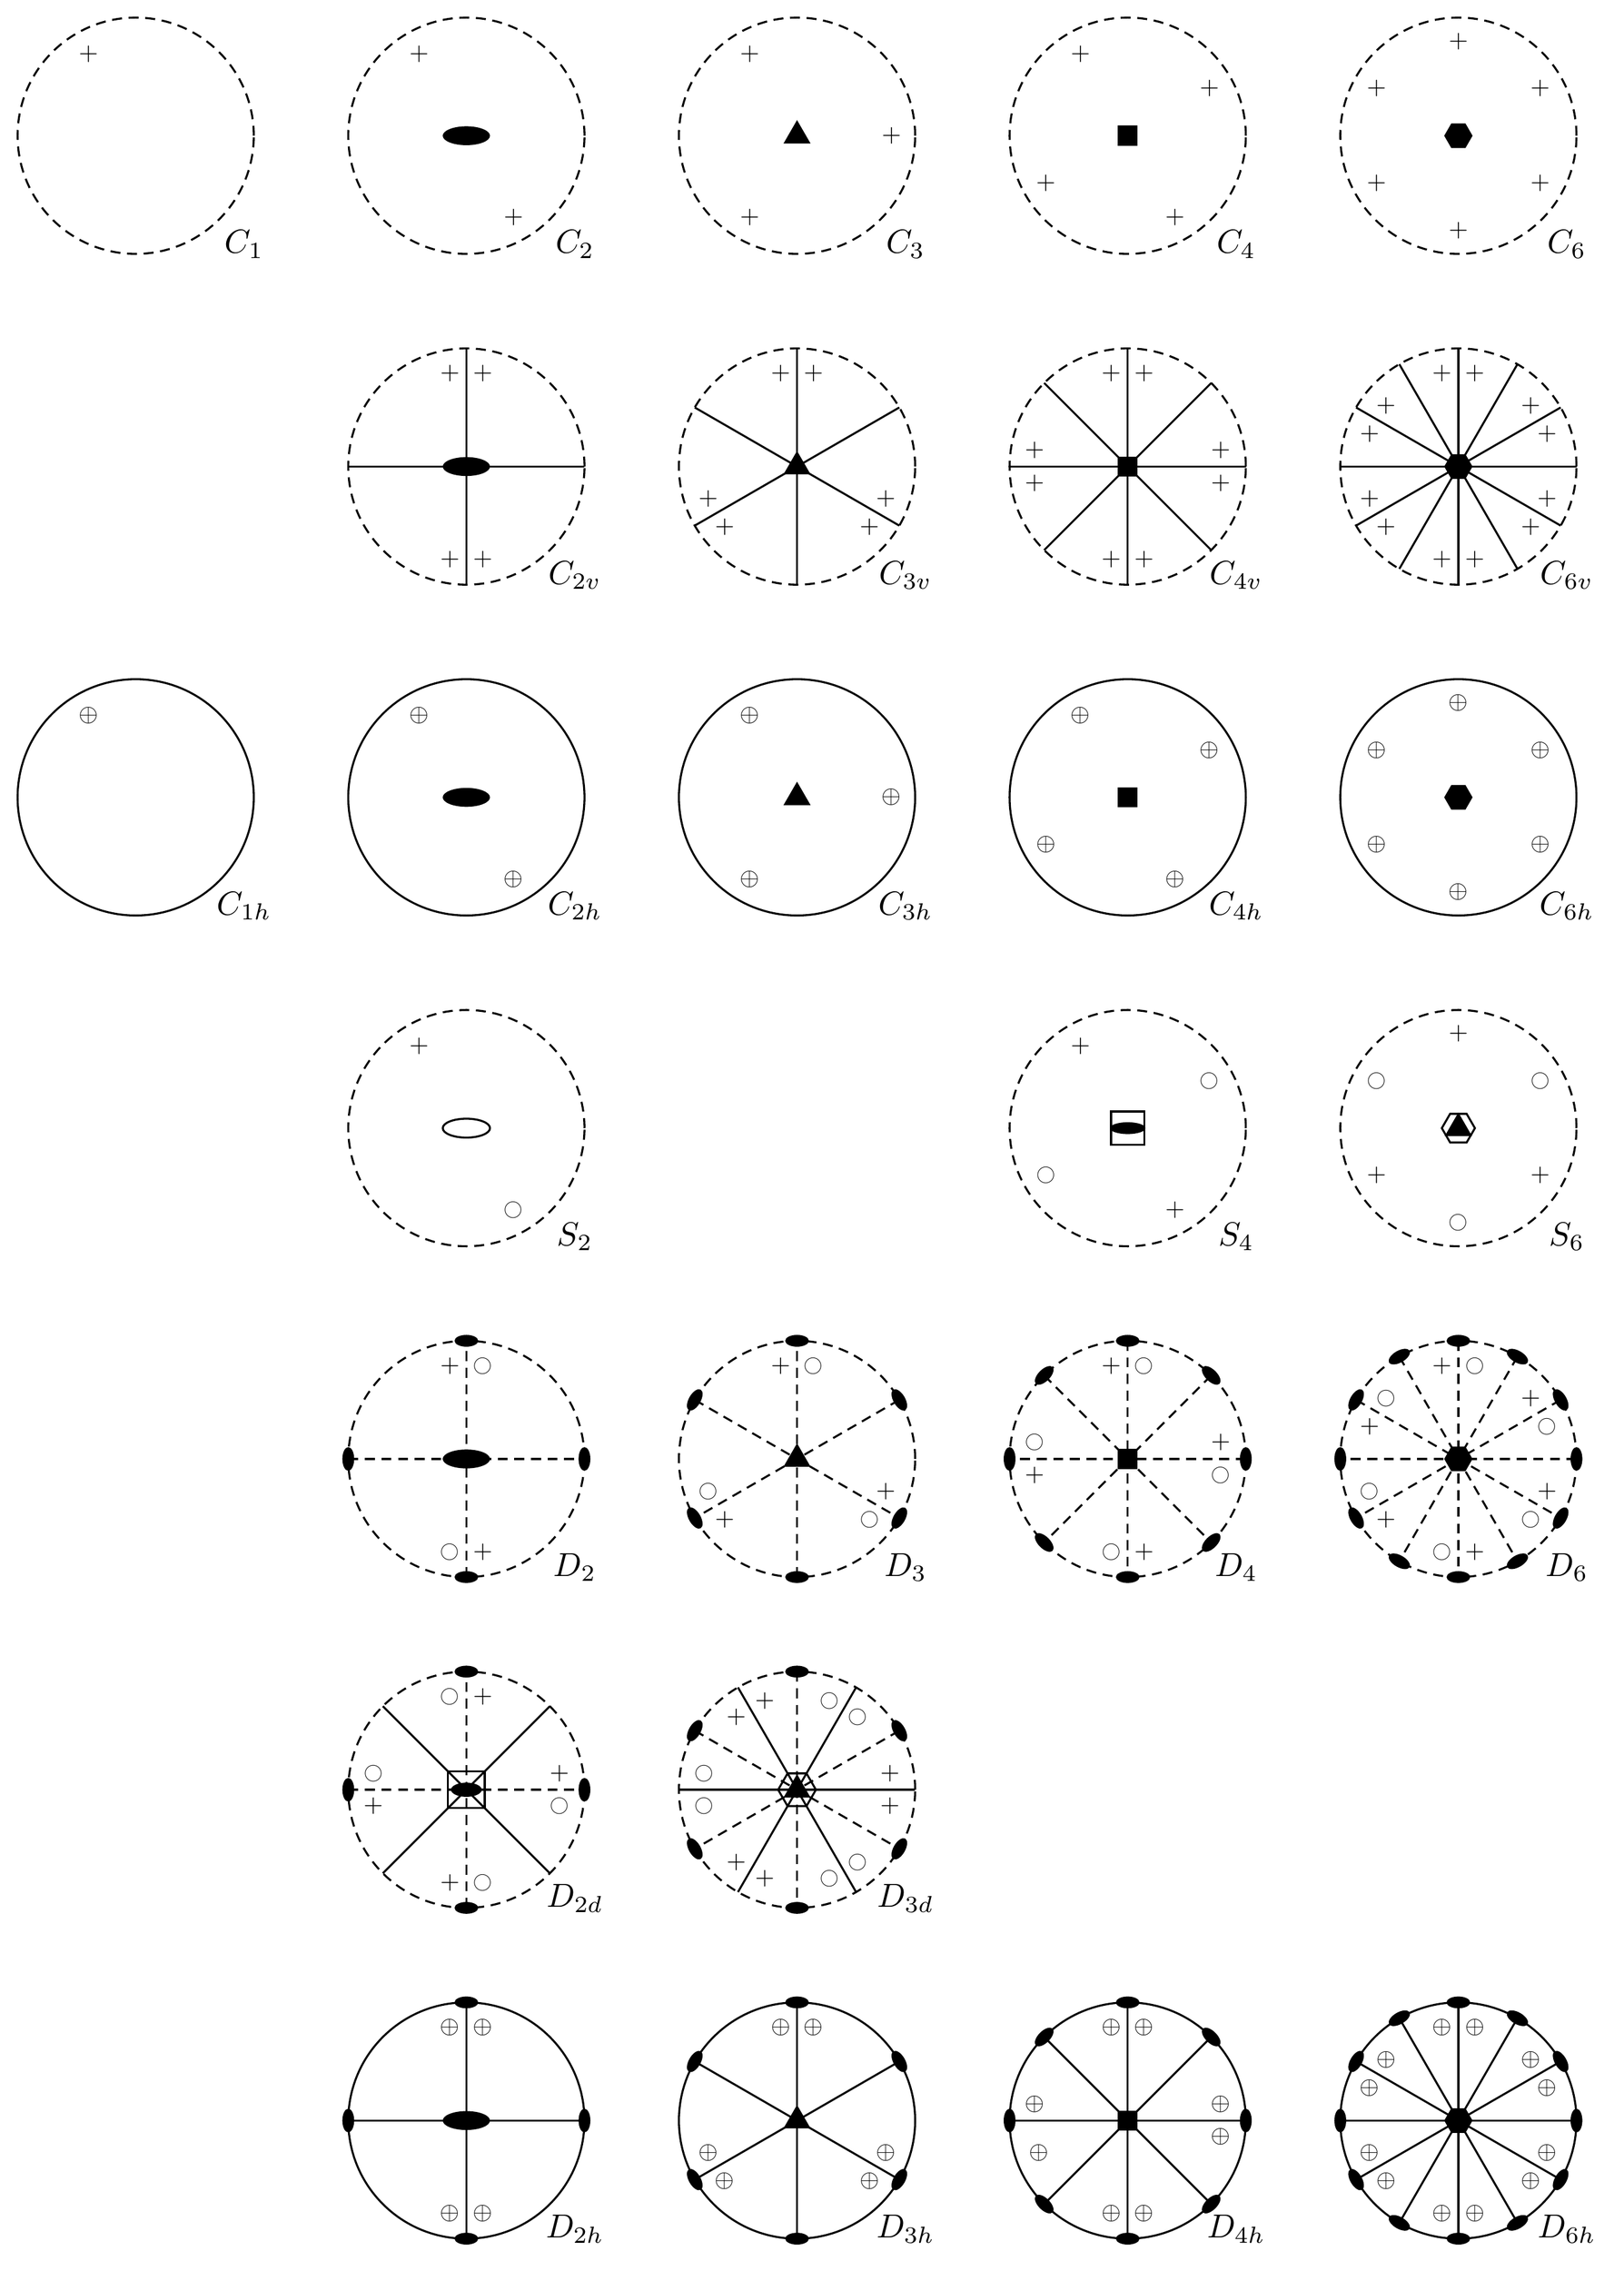
\begin{tikzpicture}[scale=2.5, extended line/.style={shorten >=-#1,shorten <=-#1},
    extended line/.default=1cm]

    \begin{scope}[]
        \def\Ra{1.3};
        \def\Rb{0.8};
        \draw[ddash, very thick](0,0) circle (1);
        \node[scale=2] at ({\Ra*cos(315)}, {\Ra*sin(315)}) {$C_1$};
        \node[scale=1.5] at ({\Rb*cos(120)}, {\Rb*sin(120)}) {$+$};
    \end{scope}

    \begin{scope}[xshift=2.8cm]
        \def\Ra{1.3};
        \def\Rb{0.8};
        \draw[ddash, very thick](0,0) circle (1);
        \node[scale=2] at ({\Ra*cos(315)}, {\Ra*sin(315)}) {$C_2$};
        \fill[] (0,0) ellipse (0.2 and 0.08);
        \node[scale=1.5] at ({\Rb*cos(120)}, {\Rb*sin(120)}) {$+$};
        \node[scale=1.5] at ({\Rb*cos(300)}, {\Rb*sin(300)}) {$+$};
    \end{scope}

    \begin{scope}[xshift=5.6cm]
        \def\Ra{1.3};
        \def\Rb{0.8};
        \draw[ddash, very thick](0,0) circle (1);
        \node[scale=2] at ({\Ra*cos(315)}, {\Ra*sin(315)}) {$C_3$};
        \node[fill,minimum size=0.5cm,regular polygon,regular polygon sides=3] at (0, 0) {};
        \node[scale=1.5] at ({\Rb*cos(120)}, {\Rb*sin(120)}) {$+$};
        \node[scale=1.5] at ({\Rb*cos(240)}, {\Rb*sin(240)}) {$+$};
        \node[scale=1.5] at ({\Rb*cos(0)}, {\Rb*sin(0)}) {$+$};
    \end{scope}

    \begin{scope}[xshift=8.4cm]
        \def\Ra{1.3};
        \def\Rb{0.8};
        \draw[ddash, very thick](0,0) circle (1);
        \node[scale=2] at ({\Ra*cos(315)}, {\Ra*sin(315)}) {$C_4$};
        \node[fill,minimum size=0.6cm,regular polygon,regular polygon sides=4] at (0, 0) {};
        \node[scale=1.5] at ({\Rb*cos(120)}, {\Rb*sin(120)}) {$+$};
        \node[scale=1.5] at ({\Rb*cos(210)}, {\Rb*sin(210)}) {$+$};
        \node[scale=1.5] at ({\Rb*cos(300)}, {\Rb*sin(300)}) {$+$};
        \node[scale=1.5] at ({\Rb*cos(30)}, {\Rb*sin(30)}) {$+$};
    \end{scope}

    \begin{scope}[xshift=11.2cm]
        \def\Ra{1.3};
        \def\Rb{0.8};
        \draw[ddash, very thick](0,0) circle (1);
        \node[scale=2] at ({\Ra*cos(315)}, {\Ra*sin(315)}) {$C_6$};
        \node[fill,minimum size=0.6cm,regular polygon,regular polygon sides=6] at (0, 0) {};
        \node[scale=1.5] at ({\Rb*cos(30)}, {\Rb*sin(30)}) {$+$};
        \node[scale=1.5] at ({\Rb*cos(90)}, {\Rb*sin(90)}) {$+$};
        \node[scale=1.5] at ({\Rb*cos(150)}, {\Rb*sin(150)}) {$+$};
        \node[scale=1.5] at ({\Rb*cos(210)}, {\Rb*sin(210)}) {$+$};
        \node[scale=1.5] at ({\Rb*cos(270)}, {\Rb*sin(270)}) {$+$};
        \node[scale=1.5] at ({\Rb*cos(330)}, {\Rb*sin(330)}) {$+$};
    \end{scope}

    \begin{scope}[xshift=2.8cm, yshift=-2.8cm]
        \def\Ra{1.3};
        \def\Rb{0.8};
        \draw[ddash, very thick](0,0) circle (1);
        \node[scale=2] at ({\Ra*cos(315)}, {\Ra*sin(315)}) {$C_{2v}$};
        \fill[] (0,0) ellipse (0.2 and 0.08);
        \draw[very thick] (-1, 0) -- (1, 0);
        \draw[very thick] (0, -1) -- (0, 1);
        \node[scale=1.5] at ({\Rb*cos(80)}, {\Rb*sin(80)}) {$+$};
        \node[scale=1.5] at ({\Rb*cos(100)}, {\Rb*sin(100)}) {$+$};
        \node[scale=1.5] at ({\Rb*cos(260)}, {\Rb*sin(260)}) {$+$};
        \node[scale=1.5] at ({\Rb*cos(280)}, {\Rb*sin(280)}) {$+$};
    \end{scope}

    \begin{scope}[xshift=5.6cm, yshift=-2.8cm]
        \def\Ra{1.3};
        \def\Rb{0.8};
        \draw[ddash, very thick](0,0) circle (1);
        \node[scale=2] at ({\Ra*cos(315)}, {\Ra*sin(315)}) {$C_{3v}$};
        \node[fill,minimum size=0.5cm,regular polygon,regular polygon sides=3] at (0, 0) {};
        \draw[very thick] (0, -1) -- (0, 1);
        \draw[very thick] ({cos(30)}, {sin(30)}) -- ({cos(210)}, {sin(210)});
        \draw[very thick] ({cos(150)}, {sin(150)}) -- ({cos(330)}, {sin(330)});
        \node[scale=1.5] at ({\Rb*cos(80)}, {\Rb*sin(80)}) {$+$};
        \node[scale=1.5] at ({\Rb*cos(100)}, {\Rb*sin(100)}) {$+$};
        \node[scale=1.5] at ({\Rb*cos(200)}, {\Rb*sin(200)}) {$+$};
        \node[scale=1.5] at ({\Rb*cos(220)}, {\Rb*sin(220)}) {$+$};
        \node[scale=1.5] at ({\Rb*cos(320)}, {\Rb*sin(320)}) {$+$};
        \node[scale=1.5] at ({\Rb*cos(340)}, {\Rb*sin(340)}) {$+$};
    \end{scope}


    \begin{scope}[xshift=8.4cm, yshift=-2.8cm]
        \def\Ra{1.3};
        \def\Rb{0.8};
        \draw[ddash, very thick](0,0) circle (1);
        \node[scale=2] at ({\Ra*cos(315)}, {\Ra*sin(315)}) {$C_{4v}$};
        \node[fill,minimum size=0.6cm,regular polygon,regular polygon sides=4] at (0, 0) {};
        \draw[very thick] ({cos(0)}, {sin(0)}) -- ({cos(180)}, {sin(180)});
        \draw[very thick] ({cos(45)}, {sin(45)}) -- ({cos(225)}, {sin(225)});
        \draw[very thick] ({cos(90)}, {sin(90)}) -- ({cos(270)}, {sin(270)});
        \draw[very thick] ({cos(135)}, {sin(135)}) -- ({cos(315)}, {sin(315)});
        \node[scale=1.5] at ({\Rb*cos(10)}, {\Rb*sin(10)}) {$+$};
        \node[scale=1.5] at ({\Rb*cos(350)}, {\Rb*sin(350)}) {$+$};
        \node[scale=1.5] at ({\Rb*cos(80)}, {\Rb*sin(80)}) {$+$};
        \node[scale=1.5] at ({\Rb*cos(100)}, {\Rb*sin(100)}) {$+$};
        \node[scale=1.5] at ({\Rb*cos(170)}, {\Rb*sin(170)}) {$+$};
        \node[scale=1.5] at ({\Rb*cos(190)}, {\Rb*sin(190)}) {$+$};
        \node[scale=1.5] at ({\Rb*cos(260)}, {\Rb*sin(260)}) {$+$};
        \node[scale=1.5] at ({\Rb*cos(280)}, {\Rb*sin(280)}) {$+$};
    \end{scope}


    \begin{scope}[xshift=11.2cm, yshift=-2.8cm]
        \def\Ra{1.3};
        \def\Rb{0.8};
        \draw[ddash, very thick](0,0) circle (1);
        \node[scale=2] at ({\Ra*cos(315)}, {\Ra*sin(315)}) {$C_{6v}$};
        \node[fill,minimum size=0.6cm,regular polygon,regular polygon sides=6] at (0, 0) {};
        \draw[very thick] ({cos(0)}, {sin(0)}) -- ({cos(180)}, {sin(180)});
        \draw[very thick] ({cos(30)}, {sin(30)}) -- ({cos(210)}, {sin(210)});
        \draw[very thick] ({cos(60)}, {sin(60)}) -- ({cos(240)}, {sin(240)});
        \draw[very thick] ({cos(90)}, {sin(90)}) -- ({cos(270)}, {sin(270)});
        \draw[very thick] ({cos(120)}, {sin(120)}) -- ({cos(300)}, {sin(300)});
        \draw[very thick] ({cos(150)}, {sin(150)}) -- ({cos(330)}, {sin(330)});
        \node[scale=1.5] at ({\Rb*cos(20)}, {\Rb*sin(20)}) {$+$};
        \node[scale=1.5] at ({\Rb*cos(40)}, {\Rb*sin(40)}) {$+$};
        \node[scale=1.5] at ({\Rb*cos(80)}, {\Rb*sin(80)}) {$+$};
        \node[scale=1.5] at ({\Rb*cos(100)}, {\Rb*sin(100)}) {$+$};
        \node[scale=1.5] at ({\Rb*cos(140)}, {\Rb*sin(140)}) {$+$};
        \node[scale=1.5] at ({\Rb*cos(160)}, {\Rb*sin(160)}) {$+$};
        \node[scale=1.5] at ({\Rb*cos(200)}, {\Rb*sin(200)}) {$+$};
        \node[scale=1.5] at ({\Rb*cos(220)}, {\Rb*sin(220)}) {$+$};
        \node[scale=1.5] at ({\Rb*cos(260)}, {\Rb*sin(260)}) {$+$};
        \node[scale=1.5] at ({\Rb*cos(280)}, {\Rb*sin(280)}) {$+$};
        \node[scale=1.5] at ({\Rb*cos(320)}, {\Rb*sin(320)}) {$+$};
        \node[scale=1.5] at ({\Rb*cos(340)}, {\Rb*sin(340)}) {$+$};
    \end{scope}

    \begin{scope}[yshift=-5.6cm]
        \def\Ra{1.3};
        \def\Rb{0.8};
        \draw[very thick](0,0) circle (1);
        \node[scale=2] at ({\Ra*cos(315)}, {\Ra*sin(315)}) {$C_{1h}$};
        \node[scale=1.5] at ({\Rb*cos(120)}, {\Rb*sin(120)}) {$\oplus$};
    \end{scope}

    \begin{scope}[xshift=2.8cm, yshift=-5.6cm]
        \def\Ra{1.3};
        \def\Rb{0.8};
        \draw[very thick](0,0) circle (1);
        \node[scale=2] at ({\Ra*cos(315)}, {\Ra*sin(315)}) {$C_{2h}$};
        \fill[] (0,0) ellipse (0.2 and 0.08);
        \node[scale=1.5] at ({\Rb*cos(120)}, {\Rb*sin(120)}) {$\oplus$};
        \node[scale=1.5] at ({\Rb*cos(300)}, {\Rb*sin(300)}) {$\oplus$};
    \end{scope}

    \begin{scope}[xshift=5.6cm, yshift=-5.6cm]
        \def\Ra{1.3};
        \def\Rb{0.8};
        \draw[very thick](0,0) circle (1);
        \node[scale=2] at ({\Ra*cos(315)}, {\Ra*sin(315)}) {$C_{3h}$};
        \node[fill,minimum size=0.5cm,regular polygon,regular polygon sides=3] at (0, 0) {};
        \node[scale=1.5] at ({\Rb*cos(120)}, {\Rb*sin(120)}) {$\oplus$};
        \node[scale=1.5] at ({\Rb*cos(240)}, {\Rb*sin(240)}) {$\oplus$};
        \node[scale=1.5] at ({\Rb*cos(0)}, {\Rb*sin(0)}) {$\oplus$};
    \end{scope}

    \begin{scope}[xshift=8.4cm, yshift=-5.6cm]
        \def\Ra{1.3};
        \def\Rb{0.8};
        \draw[very thick](0,0) circle (1);
        \node[scale=2] at ({\Ra*cos(315)}, {\Ra*sin(315)}) {$C_{4h}$};
        \node[fill,minimum size=0.6cm,regular polygon,regular polygon sides=4] at (0, 0) {};
        \node[scale=1.5] at ({\Rb*cos(120)}, {\Rb*sin(120)}) {$\oplus$};
        \node[scale=1.5] at ({\Rb*cos(210)}, {\Rb*sin(210)}) {$\oplus$};
        \node[scale=1.5] at ({\Rb*cos(300)}, {\Rb*sin(300)}) {$\oplus$};
        \node[scale=1.5] at ({\Rb*cos(30)}, {\Rb*sin(30)}) {$\oplus$};
    \end{scope}

    \begin{scope}[xshift=11.2cm, yshift=-5.6cm]
        \def\Ra{1.3};
        \def\Rb{0.8};
        \draw[very thick](0,0) circle (1);
        \node[scale=2] at ({\Ra*cos(315)}, {\Ra*sin(315)}) {$C_{6h}$};
        \node[fill,minimum size=0.6cm,regular polygon,regular polygon sides=6] at (0, 0) {};
        \node[scale=1.5] at ({\Rb*cos(30)}, {\Rb*sin(30)}) {$\oplus$};
        \node[scale=1.5] at ({\Rb*cos(90)}, {\Rb*sin(90)}) {$\oplus$};
        \node[scale=1.5] at ({\Rb*cos(150)}, {\Rb*sin(150)}) {$\oplus$};
        \node[scale=1.5] at ({\Rb*cos(210)}, {\Rb*sin(210)}) {$\oplus$};
        \node[scale=1.5] at ({\Rb*cos(270)}, {\Rb*sin(270)}) {$\oplus$};
        \node[scale=1.5] at ({\Rb*cos(330)}, {\Rb*sin(330)}) {$\oplus$};
    \end{scope}

    \begin{scope}[xshift=2.8cm, yshift=-8.4cm]
        \def\Ra{1.3};
        \def\Rb{0.8};
        \draw[ddash, very thick](0,0) circle (1);
        \node[scale=2] at ({\Ra*cos(315)}, {\Ra*sin(315)}) {$S_2$};
        \draw[very thick] (0,0) ellipse (0.2 and 0.08);
        \node[scale=1.5] at ({\Rb*cos(120)}, {\Rb*sin(120)}) {$+$};
        \node[scale=1.5] at ({\Rb*cos(300)}, {\Rb*sin(300)}) {$\Circle$};
    \end{scope}

    \begin{scope}[xshift=8.4cm, yshift=-8.4cm]
        \def\Ra{1.3};
        \def\Rb{0.8};
        \draw[ddash, very thick](0,0) circle (1);
        \node[scale=2] at ({\Ra*cos(315)}, {\Ra*sin(315)}) {$S_4$};
        \node[draw, very thick, minimum size=1cm,regular polygon,regular polygon sides=4] at (0, 0) {};
        \fill[] (0,0) ellipse (0.15 and 0.05);
        \node[scale=1.5] at ({\Rb*cos(120)}, {\Rb*sin(120)}) {$+$};
        \node[scale=1.5] at ({\Rb*cos(210)}, {\Rb*sin(210)}) {$\Circle$};
        \node[scale=1.5] at ({\Rb*cos(300)}, {\Rb*sin(300)}) {$+$};
        \node[scale=1.5] at ({\Rb*cos(30)}, {\Rb*sin(30)}) {$\Circle$};
    \end{scope}

    \begin{scope}[xshift=11.2cm, yshift=-8.4cm]
        \def\Ra{1.3};
        \def\Rb{0.8};
        \draw[ddash, very thick](0,0) circle (1);
        \node[scale=2] at ({\Ra*cos(315)}, {\Ra*sin(315)}) {$S_6$};
        \node[draw, very thick, minimum size=0.7cm,regular polygon,regular polygon sides=6] at (0, 0) {};
        \node[fill,minimum size=0.4cm,regular polygon,regular polygon sides=3] at (0, 0) {};
        \node[scale=1.5] at ({\Rb*cos(30)}, {\Rb*sin(30)}) {$\Circle$};
        \node[scale=1.5] at ({\Rb*cos(90)}, {\Rb*sin(90)}) {$+$};
        \node[scale=1.5] at ({\Rb*cos(150)}, {\Rb*sin(150)}) {$\Circle$};
        \node[scale=1.5] at ({\Rb*cos(210)}, {\Rb*sin(210)}) {$+$};
        \node[scale=1.5] at ({\Rb*cos(270)}, {\Rb*sin(270)}) {$\Circle$};
        \node[scale=1.5] at ({\Rb*cos(330)}, {\Rb*sin(330)}) {$+$};
    \end{scope}

    \begin{scope}[xshift=2.8cm, yshift=-11.2cm]
        \def\Ra{1.3};
        \def\Rb{0.8};
        \draw[ddash, very thick](0,0) circle (1);
        \node[scale=2] at ({\Ra*cos(315)}, {\Ra*sin(315)}) {$D_{2}$};
        \fill[] (0,0) ellipse (0.2 and 0.08);
        \fill[] (1,0) ellipse (0.05 and 0.1);
        \fill[] (0,1) ellipse (0.1 and 0.05);
        \fill[] (-1,0) ellipse (0.05 and 0.1);
        \fill[] (0,-1) ellipse (0.1 and 0.05);
        \draw[very thick, ddash] (-1, 0) -- (1, 0);
        \draw[very thick, ddash] (0, -1) -- (0, 1);
        \node[scale=1.5] at ({\Rb*cos(80)}, {\Rb*sin(80)}) {$\Circle$};
        \node[scale=1.5] at ({\Rb*cos(100)}, {\Rb*sin(100)}) {$+$};
        \node[scale=1.5] at ({\Rb*cos(260)}, {\Rb*sin(260)}) {$\Circle$};
        \node[scale=1.5] at ({\Rb*cos(280)}, {\Rb*sin(280)}) {$+$};
    \end{scope}

    \begin{scope}[xshift=5.6cm, yshift=-11.2cm]
        \def\Ra{1.3};
        \def\Rb{0.8};
        \draw[ddash, very thick](0,0) circle (1);
        \node[scale=2] at ({\Ra*cos(315)}, {\Ra*sin(315)}) {$D_{3}$};
        \node[fill,minimum size=0.5cm,regular polygon,regular polygon sides=3] at (0, 0) {};
        \fill[shift={({cos(30)}, {sin(30)})}, rotate=30] (0,0) ellipse (0.05 and 0.1);
        \fill[shift={({cos(90)}, {sin(90)})}, rotate=90] (0,0) ellipse (0.05 and 0.1);
        \fill[shift={({cos(150)}, {sin(150)})}, rotate=150] (0,0) ellipse (0.05 and 0.1);
        \fill[shift={({cos(210)}, {sin(210)})}, rotate=210] (0,0) ellipse (0.05 and 0.1);
        \fill[shift={({cos(270)}, {sin(270)})}, rotate=270] (0,0) ellipse (0.05 and 0.1);
        \fill[shift={({cos(330)}, {sin(330)})}, rotate=330] (0,0) ellipse (0.05 and 0.1);
        \draw[very thick, ddash] (0, -1) -- (0, 1);
        \draw[very thick, ddash] ({cos(30)}, {sin(30)}) -- ({cos(210)}, {sin(210)});
        \draw[very thick, ddash] ({cos(150)}, {sin(150)}) -- ({cos(330)}, {sin(330)});
        \node[scale=1.5] at ({\Rb*cos(80)}, {\Rb*sin(80)}) {$\Circle$};
        \node[scale=1.5] at ({\Rb*cos(100)}, {\Rb*sin(100)}) {$+$};
        \node[scale=1.5] at ({\Rb*cos(200)}, {\Rb*sin(200)}) {$\Circle$};
        \node[scale=1.5] at ({\Rb*cos(220)}, {\Rb*sin(220)}) {$+$};
        \node[scale=1.5] at ({\Rb*cos(320)}, {\Rb*sin(320)}) {$\Circle$};
        \node[scale=1.5] at ({\Rb*cos(340)}, {\Rb*sin(340)}) {$+$};
    \end{scope}


    \begin{scope}[xshift=8.4cm, yshift=-11.2cm]
        \def\Ra{1.3};
        \def\Rb{0.8};
        \draw[ddash, very thick](0,0) circle (1);
        \node[scale=2] at ({\Ra*cos(315)}, {\Ra*sin(315)}) {$D_{4}$};
        \node[fill,minimum size=0.6cm,regular polygon,regular polygon sides=4] at (0, 0) {};
        \fill[shift={({cos(0)}, {sin(0)})}, rotate=0] (0,0) ellipse (0.05 and 0.1);
        \fill[shift={({cos(45)}, {sin(45)})}, rotate=45] (0,0) ellipse (0.05 and 0.1);
        \fill[shift={({cos(90)}, {sin(90)})}, rotate=90] (0,0) ellipse (0.05 and 0.1);
        \fill[shift={({cos(135)}, {sin(135)})}, rotate=135] (0,0) ellipse (0.05 and 0.1);
        \fill[shift={({cos(180)}, {sin(180)})}, rotate=180] (0,0) ellipse (0.05 and 0.1);
        \fill[shift={({cos(225)}, {sin(225)})}, rotate=225] (0,0) ellipse (0.05 and 0.1);
        \fill[shift={({cos(270)}, {sin(270)})}, rotate=270] (0,0) ellipse (0.05 and 0.1);
        \fill[shift={({cos(315)}, {sin(315)})}, rotate=315] (0,0) ellipse (0.05 and 0.1);
        \draw[very thick, ddash] ({cos(0)}, {sin(0)}) -- ({cos(180)}, {sin(180)});
        \draw[very thick, ddash] ({cos(45)}, {sin(45)}) -- ({cos(225)}, {sin(225)});
        \draw[very thick, ddash] ({cos(90)}, {sin(90)}) -- ({cos(270)}, {sin(270)});
        \draw[very thick, ddash] ({cos(135)}, {sin(135)}) -- ({cos(315)}, {sin(315)});
        \node[scale=1.5] at ({\Rb*cos(10)}, {\Rb*sin(10)}) {$+$};
        \node[scale=1.5] at ({\Rb*cos(350)}, {\Rb*sin(350)}) {$\Circle$};
        \node[scale=1.5] at ({\Rb*cos(80)}, {\Rb*sin(80)}) {$\Circle$};
        \node[scale=1.5] at ({\Rb*cos(100)}, {\Rb*sin(100)}) {$+$};
        \node[scale=1.5] at ({\Rb*cos(170)}, {\Rb*sin(170)}) {$\Circle$};
        \node[scale=1.5] at ({\Rb*cos(190)}, {\Rb*sin(190)}) {$+$};
        \node[scale=1.5] at ({\Rb*cos(260)}, {\Rb*sin(260)}) {$\Circle$};
        \node[scale=1.5] at ({\Rb*cos(280)}, {\Rb*sin(280)}) {$+$};
    \end{scope}


    \begin{scope}[xshift=11.2cm, yshift=-11.2cm]
        \def\Ra{1.3};
        \def\Rb{0.8};
        \draw[ddash, very thick](0,0) circle (1);
        \node[scale=2] at ({\Ra*cos(315)}, {\Ra*sin(315)}) {$D_{6}$};
        \node[fill,minimum size=0.6cm,regular polygon,regular polygon sides=6] at (0, 0) {};
        \fill[shift={({cos(0)}, {sin(0)})}, rotate=0] (0,0) ellipse (0.05 and 0.1);
        \fill[shift={({cos(30)}, {sin(30)})}, rotate=30] (0,0) ellipse (0.05 and 0.1);
        \fill[shift={({cos(60)}, {sin(60)})}, rotate=60] (0,0) ellipse (0.05 and 0.1);
        \fill[shift={({cos(90)}, {sin(90)})}, rotate=90] (0,0) ellipse (0.05 and 0.1);
        \fill[shift={({cos(120)}, {sin(120)})}, rotate=120] (0,0) ellipse (0.05 and 0.1);
        \fill[shift={({cos(150)}, {sin(150)})}, rotate=150] (0,0) ellipse (0.05 and 0.1);
        \fill[shift={({cos(180)}, {sin(180)})}, rotate=180] (0,0) ellipse (0.05 and 0.1);
        \fill[shift={({cos(210)}, {sin(210)})}, rotate=210] (0,0) ellipse (0.05 and 0.1);
        \fill[shift={({cos(240)}, {sin(240)})}, rotate=240] (0,0) ellipse (0.05 and 0.1);
        \fill[shift={({cos(270)}, {sin(270)})}, rotate=270] (0,0) ellipse (0.05 and 0.1);
        \fill[shift={({cos(300)}, {sin(300)})}, rotate=300] (0,0) ellipse (0.05 and 0.1);
        \fill[shift={({cos(330)}, {sin(330)})}, rotate=330] (0,0) ellipse (0.05 and 0.1);
        \draw[very thick, ddash] ({cos(0)}, {sin(0)}) -- ({cos(180)}, {sin(180)});
        \draw[very thick, ddash] ({cos(30)}, {sin(30)}) -- ({cos(210)}, {sin(210)});
        \draw[very thick, ddash] ({cos(60)}, {sin(60)}) -- ({cos(240)}, {sin(240)});
        \draw[very thick, ddash] ({cos(90)}, {sin(90)}) -- ({cos(270)}, {sin(270)});
        \draw[very thick, ddash] ({cos(120)}, {sin(120)}) -- ({cos(300)}, {sin(300)});
        \draw[very thick, ddash] ({cos(150)}, {sin(150)}) -- ({cos(330)}, {sin(330)});
        \node[scale=1.5] at ({\Rb*cos(20)}, {\Rb*sin(20)}) {$\Circle$};
        \node[scale=1.5] at ({\Rb*cos(40)}, {\Rb*sin(40)}) {$+$};
        \node[scale=1.5] at ({\Rb*cos(80)}, {\Rb*sin(80)}) {$\Circle$};
        \node[scale=1.5] at ({\Rb*cos(100)}, {\Rb*sin(100)}) {$+$};
        \node[scale=1.5] at ({\Rb*cos(140)}, {\Rb*sin(140)}) {$\Circle$};
        \node[scale=1.5] at ({\Rb*cos(160)}, {\Rb*sin(160)}) {$+$};
        \node[scale=1.5] at ({\Rb*cos(200)}, {\Rb*sin(200)}) {$\Circle$};
        \node[scale=1.5] at ({\Rb*cos(220)}, {\Rb*sin(220)}) {$+$};
        \node[scale=1.5] at ({\Rb*cos(260)}, {\Rb*sin(260)}) {$\Circle$};
        \node[scale=1.5] at ({\Rb*cos(280)}, {\Rb*sin(280)}) {$+$};
        \node[scale=1.5] at ({\Rb*cos(320)}, {\Rb*sin(320)}) {$\Circle$};
        \node[scale=1.5] at ({\Rb*cos(340)}, {\Rb*sin(340)}) {$+$};
    \end{scope}


    \begin{scope}[xshift=2.8cm, yshift=-14cm]
        \def\Ra{1.3};
        \def\Rb{0.8};
        \draw[ddash, very thick](0,0) circle (1);
        \node[scale=2] at ({\Ra*cos(315)}, {\Ra*sin(315)}) {$D_{2d}$};
        \fill[] (0,0) ellipse (0.13 and 0.06);
        \node[draw, very thick, minimum size=1.1cm,regular polygon,regular polygon sides=4] at (0, 0) {};
        \fill[] (1,0) ellipse (0.05 and 0.1);
        \fill[] (0,1) ellipse (0.1 and 0.05);
        \fill[] (-1,0) ellipse (0.05 and 0.1);
        \fill[] (0,-1) ellipse (0.1 and 0.05);
        \draw[very thick, ddash] (-1, 0) -- (1, 0);
        \draw[very thick, ddash] (0, -1) -- (0, 1);
        \draw[very thick] ({cos(45)}, {sin(45)}) -- ({cos(225)}, {sin(225)});
        \draw[very thick] ({cos(135)}, {sin(135)}) -- ({cos(315)}, {sin(315)});
        \node[scale=1.5] at ({\Rb*cos(350)}, {\Rb*sin(350)}) {$\Circle$};
        \node[scale=1.5] at ({\Rb*cos(10)}, {\Rb*sin(10)}) {$+$};
        \node[scale=1.5] at ({\Rb*cos(80)}, {\Rb*sin(80)}) {$+$};
        \node[scale=1.5] at ({\Rb*cos(100)}, {\Rb*sin(100)}) {$\Circle$};
        \node[scale=1.5] at ({\Rb*cos(170)}, {\Rb*sin(170)}) {$\Circle$};
        \node[scale=1.5] at ({\Rb*cos(190)}, {\Rb*sin(190)}) {$+$};
        \node[scale=1.5] at ({\Rb*cos(260)}, {\Rb*sin(260)}) {$+$};
        \node[scale=1.5] at ({\Rb*cos(280)}, {\Rb*sin(280)}) {$\Circle$};
    \end{scope}

    \begin{scope}[xshift=5.6cm, yshift=-14cm]
        \def\Ra{1.3};
        \def\Rb{0.8};
        \draw[ddash, very thick](0,0) circle (1);
        \node[scale=2] at ({\Ra*cos(315)}, {\Ra*sin(315)}) {$D_{3d}$};
        \node[fill,minimum size=0.6cm,regular polygon,regular polygon sides=3] at (0, 0) {};
        \node[draw, very thick, minimum size=0.8cm,regular polygon,regular polygon sides=6] at (0, 0) {};
        \fill[shift={({cos(30)}, {sin(30)})}, rotate=30] (0,0) ellipse (0.05 and 0.1);
        \fill[shift={({cos(90)}, {sin(90)})}, rotate=90] (0,0) ellipse (0.05 and 0.1);
        \fill[shift={({cos(150)}, {sin(150)})}, rotate=150] (0,0) ellipse (0.05 and 0.1);
        \fill[shift={({cos(210)}, {sin(210)})}, rotate=210] (0,0) ellipse (0.05 and 0.1);
        \fill[shift={({cos(270)}, {sin(270)})}, rotate=270] (0,0) ellipse (0.05 and 0.1);
        \fill[shift={({cos(330)}, {sin(330)})}, rotate=330] (0,0) ellipse (0.05 and 0.1);
        \draw[very thick] ({cos(0)}, {sin(0)}) -- ({cos(180)}, {sin(180)});
        \draw[very thick, ddash] ({cos(30)}, {sin(30)}) -- ({cos(210)}, {sin(210)});
        \draw[very thick] ({cos(60)}, {sin(60)}) -- ({cos(240)}, {sin(240)});
        \draw[very thick, ddash] ({cos(90)}, {sin(90)}) -- ({cos(270)}, {sin(270)});
        \draw[very thick] ({cos(120)}, {sin(120)}) -- ({cos(300)}, {sin(300)});
        \draw[very thick, ddash] ({cos(150)}, {sin(150)}) -- ({cos(330)}, {sin(330)});
        \node[scale=1.5] at ({\Rb*cos(350)}, {\Rb*sin(350)}) {$+$};
        \node[scale=1.5] at ({\Rb*cos(10)}, {\Rb*sin(10)}) {$+$};
        \node[scale=1.5] at ({\Rb*cos(50)}, {\Rb*sin(50)}) {$\Circle$};
        \node[scale=1.5] at ({\Rb*cos(70)}, {\Rb*sin(70)}) {$\Circle$};
        \node[scale=1.5] at ({\Rb*cos(110)}, {\Rb*sin(110)}) {$+$};
        \node[scale=1.5] at ({\Rb*cos(130)}, {\Rb*sin(130)}) {$+$};
        \node[scale=1.5] at ({\Rb*cos(170)}, {\Rb*sin(170)}) {$\Circle$};
        \node[scale=1.5] at ({\Rb*cos(190)}, {\Rb*sin(190)}) {$\Circle$};
        \node[scale=1.5] at ({\Rb*cos(230)}, {\Rb*sin(230)}) {$+$};
        \node[scale=1.5] at ({\Rb*cos(250)}, {\Rb*sin(250)}) {$+$};
        \node[scale=1.5] at ({\Rb*cos(290)}, {\Rb*sin(290)}) {$\Circle$};
        \node[scale=1.5] at ({\Rb*cos(310)}, {\Rb*sin(310)}) {$\Circle$};
    \end{scope}


    \begin{scope}[xshift=2.8cm, yshift=-16.8cm]
        \def\Ra{1.3};
        \def\Rb{0.8};
        \draw[very thick](0,0) circle (1);
        \node[scale=2] at ({\Ra*cos(315)}, {\Ra*sin(315)}) {$D_{2h}$};
        \fill[] (0,0) ellipse (0.2 and 0.08);
        \fill[] (1,0) ellipse (0.05 and 0.1);
        \fill[] (0,1) ellipse (0.1 and 0.05);
        \fill[] (-1,0) ellipse (0.05 and 0.1);
        \fill[] (0,-1) ellipse (0.1 and 0.05);
        \draw[very thick] (-1, 0) -- (1, 0);
        \draw[very thick] (0, -1) -- (0, 1);
        \node[scale=1.5] at ({\Rb*cos(80)}, {\Rb*sin(80)}) {$\oplus$};
        \node[scale=1.5] at ({\Rb*cos(100)}, {\Rb*sin(100)}) {$\oplus$};
        \node[scale=1.5] at ({\Rb*cos(260)}, {\Rb*sin(260)}) {$\oplus$};
        \node[scale=1.5] at ({\Rb*cos(280)}, {\Rb*sin(280)}) {$\oplus$};
    \end{scope}

    \begin{scope}[xshift=5.6cm, yshift=-16.8cm]
        \def\Ra{1.3};
        \def\Rb{0.8};
        \draw[very thick](0,0) circle (1);
        \node[scale=2] at ({\Ra*cos(315)}, {\Ra*sin(315)}) {$D_{3h}$};
        \node[fill,minimum size=0.5cm,regular polygon,regular polygon sides=3] at (0, 0) {};
        \fill[shift={({cos(30)}, {sin(30)})}, rotate=30] (0,0) ellipse (0.05 and 0.1);
        \fill[shift={({cos(90)}, {sin(90)})}, rotate=90] (0,0) ellipse (0.05 and 0.1);
        \fill[shift={({cos(150)}, {sin(150)})}, rotate=150] (0,0) ellipse (0.05 and 0.1);
        \fill[shift={({cos(210)}, {sin(210)})}, rotate=210] (0,0) ellipse (0.05 and 0.1);
        \fill[shift={({cos(270)}, {sin(270)})}, rotate=270] (0,0) ellipse (0.05 and 0.1);
        \fill[shift={({cos(330)}, {sin(330)})}, rotate=330] (0,0) ellipse (0.05 and 0.1);
        \draw[very thick] (0, -1) -- (0, 1);
        \draw[very thick] ({cos(30)}, {sin(30)}) -- ({cos(210)}, {sin(210)});
        \draw[very thick] ({cos(150)}, {sin(150)}) -- ({cos(330)}, {sin(330)});
        \node[scale=1.5] at ({\Rb*cos(80)}, {\Rb*sin(80)}) {$\oplus$};
        \node[scale=1.5] at ({\Rb*cos(100)}, {\Rb*sin(100)}) {$\oplus$};
        \node[scale=1.5] at ({\Rb*cos(200)}, {\Rb*sin(200)}) {$\oplus$};
        \node[scale=1.5] at ({\Rb*cos(220)}, {\Rb*sin(220)}) {$\oplus$};
        \node[scale=1.5] at ({\Rb*cos(320)}, {\Rb*sin(320)}) {$\oplus$};
        \node[scale=1.5] at ({\Rb*cos(340)}, {\Rb*sin(340)}) {$\oplus$};
    \end{scope}


    \begin{scope}[xshift=8.4cm, yshift=-16.8cm]
        \def\Ra{1.3};
        \def\Rb{0.8};
        \draw[very thick](0,0) circle (1);
        \node[scale=2] at ({\Ra*cos(315)}, {\Ra*sin(315)}) {$D_{4h}$};
        \node[fill,minimum size=0.6cm,regular polygon,regular polygon sides=4] at (0, 0) {};
        \fill[shift={({cos(0)}, {sin(0)})}, rotate=0] (0,0) ellipse (0.05 and 0.1);
        \fill[shift={({cos(45)}, {sin(45)})}, rotate=45] (0,0) ellipse (0.05 and 0.1);
        \fill[shift={({cos(90)}, {sin(90)})}, rotate=90] (0,0) ellipse (0.05 and 0.1);
        \fill[shift={({cos(135)}, {sin(135)})}, rotate=135] (0,0) ellipse (0.05 and 0.1);
        \fill[shift={({cos(180)}, {sin(180)})}, rotate=180] (0,0) ellipse (0.05 and 0.1);
        \fill[shift={({cos(225)}, {sin(225)})}, rotate=225] (0,0) ellipse (0.05 and 0.1);
        \fill[shift={({cos(270)}, {sin(270)})}, rotate=270] (0,0) ellipse (0.05 and 0.1);
        \fill[shift={({cos(315)}, {sin(315)})}, rotate=315] (0,0) ellipse (0.05 and 0.1);
        \draw[very thick] ({cos(0)}, {sin(0)}) -- ({cos(180)}, {sin(180)});
        \draw[very thick] ({cos(45)}, {sin(45)}) -- ({cos(225)}, {sin(225)});
        \draw[very thick] ({cos(90)}, {sin(90)}) -- ({cos(270)}, {sin(270)});
        \draw[very thick] ({cos(135)}, {sin(135)}) -- ({cos(315)}, {sin(315)});
        \node[scale=1.5] at ({\Rb*cos(10)}, {\Rb*sin(10)}) {$\oplus$};
        \node[scale=1.5] at ({\Rb*cos(350)}, {\Rb*sin(350)}) {$\oplus$};
        \node[scale=1.5] at ({\Rb*cos(80)}, {\Rb*sin(80)}) {$\oplus$};
        \node[scale=1.5] at ({\Rb*cos(100)}, {\Rb*sin(100)}) {$\oplus$};
        \node[scale=1.5] at ({\Rb*cos(170)}, {\Rb*sin(170)}) {$\oplus$};
        \node[scale=1.5] at ({\Rb*cos(200)}, {\Rb*sin(200)}) {$\oplus$};
        \node[scale=1.5] at ({\Rb*cos(260)}, {\Rb*sin(260)}) {$\oplus$};
        \node[scale=1.5] at ({\Rb*cos(280)}, {\Rb*sin(280)}) {$\oplus$};
    \end{scope}


    \begin{scope}[xshift=11.2cm, yshift=-16.8cm]
        \def\Ra{1.3};
        \def\Rb{0.8};
        \draw[very thick](0,0) circle (1);
        \node[scale=2] at ({\Ra*cos(315)}, {\Ra*sin(315)}) {$D_{6h}$};
        \node[fill,minimum size=0.6cm,regular polygon,regular polygon sides=6] at (0, 0) {};
        \fill[shift={({cos(0)}, {sin(0)})}, rotate=0] (0,0) ellipse (0.05 and 0.1);
        \fill[shift={({cos(30)}, {sin(30)})}, rotate=30] (0,0) ellipse (0.05 and 0.1);
        \fill[shift={({cos(60)}, {sin(60)})}, rotate=60] (0,0) ellipse (0.05 and 0.1);
        \fill[shift={({cos(90)}, {sin(90)})}, rotate=90] (0,0) ellipse (0.05 and 0.1);
        \fill[shift={({cos(120)}, {sin(120)})}, rotate=120] (0,0) ellipse (0.05 and 0.1);
        \fill[shift={({cos(150)}, {sin(150)})}, rotate=150] (0,0) ellipse (0.05 and 0.1);
        \fill[shift={({cos(180)}, {sin(180)})}, rotate=180] (0,0) ellipse (0.05 and 0.1);
        \fill[shift={({cos(210)}, {sin(210)})}, rotate=210] (0,0) ellipse (0.05 and 0.1);
        \fill[shift={({cos(240)}, {sin(240)})}, rotate=240] (0,0) ellipse (0.05 and 0.1);
        \fill[shift={({cos(270)}, {sin(270)})}, rotate=270] (0,0) ellipse (0.05 and 0.1);
        \fill[shift={({cos(300)}, {sin(300)})}, rotate=300] (0,0) ellipse (0.05 and 0.1);
        \fill[shift={({cos(330)}, {sin(330)})}, rotate=330] (0,0) ellipse (0.05 and 0.1);
        \draw[very thick] ({cos(0)}, {sin(0)}) -- ({cos(180)}, {sin(180)});
        \draw[very thick] ({cos(30)}, {sin(30)}) -- ({cos(210)}, {sin(210)});
        \draw[very thick] ({cos(60)}, {sin(60)}) -- ({cos(240)}, {sin(240)});
        \draw[very thick] ({cos(90)}, {sin(90)}) -- ({cos(270)}, {sin(270)});
        \draw[very thick] ({cos(120)}, {sin(120)}) -- ({cos(300)}, {sin(300)});
        \draw[very thick] ({cos(150)}, {sin(150)}) -- ({cos(330)}, {sin(330)});
        \node[scale=1.5] at ({\Rb*cos(20)}, {\Rb*sin(20)}) {$\oplus$};
        \node[scale=1.5] at ({\Rb*cos(40)}, {\Rb*sin(40)}) {$\oplus$};
        \node[scale=1.5] at ({\Rb*cos(80)}, {\Rb*sin(80)}) {$\oplus$};
        \node[scale=1.5] at ({\Rb*cos(100)}, {\Rb*sin(100)}) {$\oplus$};
        \node[scale=1.5] at ({\Rb*cos(140)}, {\Rb*sin(140)}) {$\oplus$};
        \node[scale=1.5] at ({\Rb*cos(160)}, {\Rb*sin(160)}) {$\oplus$};
        \node[scale=1.5] at ({\Rb*cos(200)}, {\Rb*sin(200)}) {$\oplus$};
        \node[scale=1.5] at ({\Rb*cos(220)}, {\Rb*sin(220)}) {$\oplus$};
        \node[scale=1.5] at ({\Rb*cos(260)}, {\Rb*sin(260)}) {$\oplus$};
        \node[scale=1.5] at ({\Rb*cos(280)}, {\Rb*sin(280)}) {$\oplus$};
        \node[scale=1.5] at ({\Rb*cos(320)}, {\Rb*sin(320)}) {$\oplus$};
        \node[scale=1.5] at ({\Rb*cos(340)}, {\Rb*sin(340)}) {$\oplus$};
    \end{scope}
\end{tikzpicture}
\end{document}